% !TeX root = ../../main.tex
\subsection{工具总体结构设计}
\label{duogongnengguolv}
多功能过滤工具\footnote{下文简称为“过滤工具”}是井筒高效清洁配套工具中的关键工具之一，由钻杆送入井下，在起钻过程中对井下钻井液进行过滤，分离并收集井底碎屑。其过滤功能独立于其他井下作业，不会影响正常下钻及循环。停泵上提过程中，该工具处于工作状态，扶正套筒移动并打开工具内部通道口，钻井液经工具内部的过滤外筒过滤后下行。

多功能过滤工具采用扶正套筒开关设计：下入时，扶正套筒关闭工具内部通道口，不影响工具串正常下钻及作业；上提时，扶正套筒打开工具内部通道口，过滤工具开始工作。

多功能过滤工具设置有观察孔及清理盖板：观察孔便于检查碎屑的收集量；清理盖板在工具作业完成后即可拆卸，以清理储存的碎屑，无需拆卸工具本体。

多功能过滤工具的结构如图~\ref{fig:filter_tool_structure}所示，主要由提升短节、上扶正套筒、扶正块、滤进接头、过滤套筒、过滤外筒、过滤内筒、清理盖板、滤出接头、下扶正套筒和下接头组成。其中，过滤套筒、过滤外筒和过滤内筒可替换为加长版，以增大过滤容量。

其工作原理为：工具下井后，扶正套筒受力上行，关闭工具内部通道口，此时过滤工具不工作，工具串可进行正常作业；当工具串上提时，扶正套筒受力下行，打开工具内部通道口，过滤工具开始工作。带有碎屑的钻井液进入工具内部，由过滤外筒完成过滤，经过滤内筒循环回井内。

\begin{figure}[htbp]
  \centering % 图片居中
  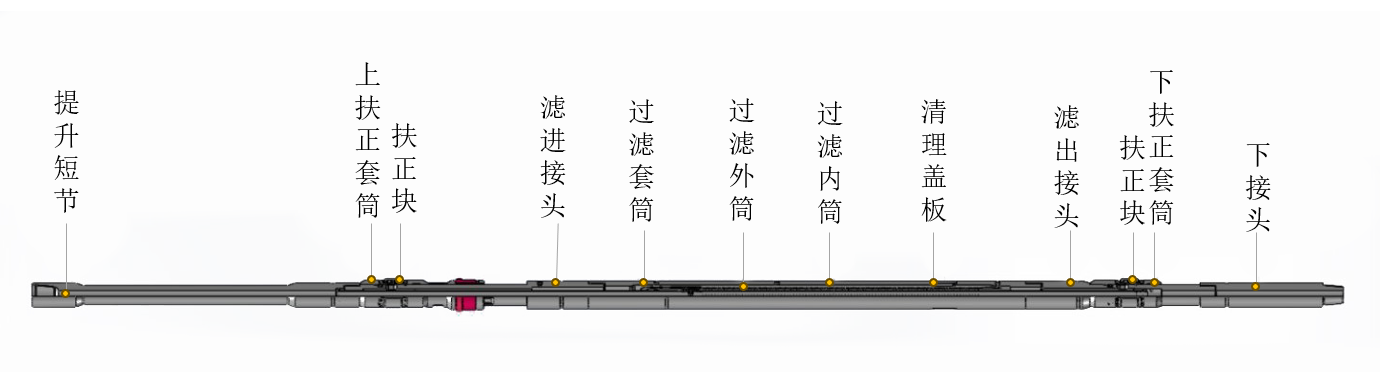
\includegraphics[width=1.0\textwidth]{figure/chapter3/guolvqi.png} % 图片路径
  \caption{多功能过滤工具结构示意图} % 图标题
  \label{fig:filter_tool_structure} % 标签，用于文中引用
\end{figure}

过滤工具的主要技术参数见表~\ref{tab:filter_tool_params}。

\begin{table}[htbp]
    \centering
    \caption{多功能过滤工具技术参数表}
    \label{tab:filter_tool_params}
    \footnotesize % 共 11 列，缩小字号以适应宽表格
    \setlength{\tabcolsep}{3pt} % 减小列间距，避免超出正文版心
    \renewcommand{\arraystretch}{1.3} % 增加行高
    
    \begin{tabularx}{\textwidth}{Xcccccccccc}
        \toprule
        型号 & 
        \begin{tabular}[c]{@{}c@{}}适用\\套管\\(in)\end{tabular} & 
        上部扣型 & 
        下部扣型 & 
        \begin{tabular}[c]{@{}c@{}}长度\\(mm)\end{tabular}& 
        \begin{tabular}[c]{@{}c@{}}本体\\外径\\(mm)\end{tabular}& 
        \begin{tabular}[c]{@{}c@{}}本体\\内径\\(mm)\end{tabular}& 
        \begin{tabular}[c]{@{}c@{}}许用抗拉\\强度\\(kN)\end{tabular}& 
        \begin{tabular}[c]{@{}c@{}}许用抗扭\\强度\\(kN$\cdot$m)\end{tabular} & 
        \begin{tabular}[c]{@{}c@{}}最大\\转数\\(rpm)\end{tabular} & 
        \begin{tabular}[c]{@{}c@{}}碎屑存储量\\(L)\end{tabular} \\
        \midrule
        
        GLGJ70000A & 7 & NC38 & NC38 & 6500 & 139.7 & 35.06 & 2500 & 39 & 120 & 6.90 \\
        
        \midrule
        
        \begin{tabular}[c]{@{}c@{}}GLGJ70000A-\\加长版\end{tabular} & 7 & NC38 & NC38 & 8786.24 & 139.7 & 35.06 & 2500 & 39 & 120 & 15.85 \\
        \bottomrule
    \end{tabularx}
\end{table}

注：表中"本体外径"为计入上、下扶正套筒后的工具最大外径，取139.7\,mm（接头及筒体本体外径为$\phi 120.65$，见图纸GLGJ70001A--上接头、GLGJ70015A）；"本体内径"指工具的最小过流内径，取零件图GLGJ70018A加长过滤内筒的内孔尺寸$\phi 35.05\pm 0.25\,\text{mm}$（滤进接头、滤出接头、下接头等接头处的内孔分别为$\phi 45.72$、$\phi 44.45$、$\phi 44.45\,\text{mm}$，见图GLGJ70002A、GLGJ70013A、GLGJ70015A）；"碎屑存储量"为按过滤腔容积并计入滤网孔隙率后的有效存储量。表中数据为 7\inch 工具（GLGJ70000A）的规格。



\subsubsection{与国外同类过滤工具的对比分析}
\label{sec:filter_tool_compare}

目前国外具有代表性的钻柱过滤工具为 Schlumberger／M-I SWACO 公司的 MUDGARD 工作管柱过滤器，同类型工具还有 Weatherford 公司的 MK3 型 Clearmax 过滤工具。MUDGARD 工具串接于钻柱之中随钻使用，在下钻、循环与起钻过程中对钻井液进行过滤，用于保护 MWD、LWD、旋转导向系统及钻头等下部钻具组合部件；据其公开产品样本，该工具采用整体式高强度筒体、无内部连接，设有应急中心旁通，可在不起出钻柱部件的条件下建立完整的钢丝作业通道，并在碎屑量超出预期、大容量滤网被堵塞时重新建立过流通道；其滤网具有抗冲蚀、流通面积大的特点，并经计算流体力学优化以尽可能减小系统压耗。MK3 型 Clearmax 过滤工具随钻具一同入井，正常下钻与循环工况下过滤机构保持关闭、不改变流体流通通道，停泵上提时触发开启，并设有破裂盘与清理盖板。上述工具与本工具的技术特点对比见表~\ref{tab:filter_tool_compare}。

\begin{table}[htbp]
    \centering
    \caption{本过滤工具与国外同类过滤工具的技术特点对比}
    \label{tab:filter_tool_compare}
    \footnotesize
    \setlength{\tabcolsep}{4pt}
    \renewcommand{\arraystretch}{1.3}
    \begin{tabularx}{\textwidth}{lXX}
        \toprule
        对比项目 & MUDGARD 工作管柱过滤器 & 本多功能过滤工具 \\
        \midrule
        过滤触发方式 & 串接于钻柱中随钻使用，对钻井液全时过滤 & 下钻时过滤机构关闭、停泵上提时触发开启的按需过滤 \\
        \midrule
        对循环压耗的影响 & 全时过流，虽经计算流体力学优化，压耗在全部钻进工况下长期存在 & 正常下钻与循环工况下内部通道口关闭，不改变流体流通通道，无附加压降 \\
        \midrule
        堵塞保护方式 & 设应急中心旁通，需配合相应作业重新建立过流通道 & 破裂盘达设定压差自动开启旁通，过滤功能自动暂停，避免工具憋压 \\
        \midrule
        容量与扩容方式 & 整体式筒体，过滤容量由筒体结构确定 & 过滤套筒、过滤外筒、过滤内筒三件可换装，加长版碎屑存储量由 $6.90\,\text{L}$ 增至 $15.85\,\text{L}$（总长由 $6500\,\text{mm}$ 增至 $8786.24\,\text{mm}$） \\
        \midrule
        内部通道 & 中心旁通用于应急钢丝作业通道 & 内通径按套管规格系列化设计，7\inch 规格为 $\phi 35.05\,\text{mm}$，9-5/8\inch 规格为 $\phi 68.28\,\text{mm}$ \\
        \midrule
        检修方式 & 样本未详细说明 & 观察孔可直接检查碎屑收集量，拆卸清理盖板即可清屑，无需拆卸工具本体 \\
        \midrule
        旋转工况 & 样本未给出允许转速 & 工具可随钻柱旋转，允许转速 $\ge 120\,\text{rpm}$ \\
        \midrule
        强度设计校核 & 样本未给出 & 完成 7 处危险截面的抗拉、抗扭校核，3.625\inch-8 Stub ACME 螺纹牙剪切 $1690.26\,\text{kN}$，NC38 接头螺纹牙剪切 $2764.1\,\text{kN}$，许用抗拉 $2500\,\text{kN}$、许用抗扭 $39\,\text{kN}\cdot\text{m}$，有限元复核安全系数 $1.56$—$1.86$ \\
        \bottomrule
    \end{tabularx}
\end{table}

注：表中 MUDGARD 工具的相关数据引自其公开产品样本，仅用于技术特点的对比说明。

\begin{figure}[htbp]
    \centering
    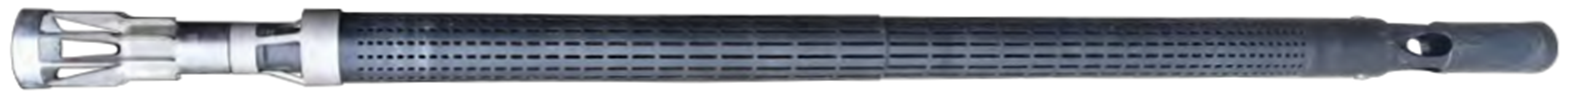
\includegraphics[width=0.95\textwidth]{figure/chapter3/mudgard-filter-tool.png}
    \caption{MUDGARD 工作管柱过滤器外形（图片来源：公开产品样本）}
    \label{fig:mudgard_tool}
\end{figure}

与上述参照工具相比，本工具的设计优势主要体现在以下几个方面。

（1）按需过滤，正常作业不产生附加压降。本工具在下钻及正常循环工况下，扶正套筒关闭工具内部通道口，钻井液不经过滤机构，工具的接入不改变原有循环通道、不产生附加压降；只有在停泵上提、进入清洁作业阶段时才打开内部通道口开始过滤。参照工具串接于钻柱中全时过流，其压耗在全部钻进工况下长期存在。

（2）堵塞后自动泄压，避免憋压风险。当储屑腔内碎屑积满、滤网内外压差达到设定值时，本工具的破裂盘受压开启，过滤功能自动暂停并使钻井液恢复循环，无需地面干预与额外作业；参照工具的应急中心旁通主要用于建立应急钢丝作业通道，其过流通道的重新建立需配合相应的井下作业。

（3）容积可按作业需求换装调整，单支工具多井复用。本工具只需更换过滤套筒、过滤外筒、过滤内筒三个零件，即可在标准版与加长版之间切换，碎屑存储量由 $6.90\,\text{L}$ 增至 $15.85\,\text{L}$，同一支工具可适配同规格不同磅级的套管，实现单支工具多井复用，降低井下作业配套工具成本。

（4）免拆解检修，运行状态可直观检查。工具设有观察孔与清理盖板，起出井口后可直接通过观察孔检查碎屑收集量，拆卸清理盖板即可清理积存的碎屑，无需对工具本体进行整体拆解。

（5）主要受力件强度校核完整。本工具对提升短节、滤进接头、滤出接头、下接头等主要受力件的连接螺纹（3.625\inch-8 Stub ACME）进行了牙剪切、根部拉伸与抗扭强度计算，对 7 处危险截面进行了校核并开展了有限元复核，安全系数为 $1.56\sim 1.86$，工具可随钻柱旋转（允许转速 $\ge 120\,\text{rpm}$）。

\subsection{过滤工具设计计算与校核}
\subsubsection{主要受力件的螺纹强度校核}

过滤工具的主要受力件为提升短节、滤进接头、滤出接头和下接头，其连接螺纹均为 3.625\inch-8 Stub ACME（材料 4145H，图纸GLGJ70001A--上接头、GLGJ70002A、GLGJ70013A、GLGJ70015A技术要求均为：调质后屈服强度$\ge 930$\,MPa、抗拉强度$\ge 1080$\,MPa）。

螺纹牙的剪切强度按下式计算：
\begin{equation}
    \begin{aligned}
        F_{\max} &= [\tau] \cdot k_z \cdot \pi \cdot d_1 \cdot b \cdot z \cdot 10^{-3} \\
        [\tau] &= \frac{\sigma_{\mathrm{s}}}{n}
    \end{aligned}
\end{equation}
式中，$F_{\max}$---工具最大拉力，kN（设计指标 $\ge 1000$\,kN，即合同条款 5.2.1.3 规定的抗拉 $\ge 100$\,T）；

$[\tau]$---螺纹牙的许用剪切强度，MPa（按 $[\tau]=\sigma_{\mathrm{s}}/n$ 计算）；

$k_z$---螺纹各圈的载荷不均系数，取 $k_z = 0.56$（按《机械设计手册》螺纹连接（紧固件连接）部分中螺纹牙的剪切强度计算及各圈螺纹载荷分配的规定\cite{ref26}）；

$d_1$---螺纹底径，取 89.66\,mm（图号 GLGJ70002A--滤进接头\ 主视图标注的 3.625\inch -8 Stub ACME 外螺纹小径 $\phi 89.100\sim \phi 89.660$ mm，取大值）；

$b$---螺纹牙根宽度，取 $b = 1.310\,\text{mm}$（按 ASME B1.8 规定的 ACME 牙型，由螺距 $p=25.4/8=3.175\,\text{mm}$ 与基本牙型高度 $h_0=p/2=1.588\,\text{mm}$ 计算）；

$z$---旋合圈数，取 $z = 22$（图号 GLGJ70002A--滤进接头外螺纹、GLGJ70001A--上接头内螺纹的旋合长度标注除以螺距 3.175\,mm 折合）；

$\sigma_{\mathrm{s}}$---材料最小屈服强度，取 930\,MPa（图号 GLGJ70001A--上接头、GLGJ70002A--滤进接头、GLGJ70013A--滤出接头、GLGJ70015A--下接头技术要求：材料 4145H，调质后屈服强度 $\ge 930$\,MPa、抗拉强度 $\ge 1080$\,MPa）；

$n$---安全系数，取 $n = 2.5$（按《机械设计手册》螺纹连接部分中螺纹牙强度校核的安全系数取值规定\cite{ref26}）。

将 3.625\inch-8 Stub ACME 螺纹的相关参数代入，计算得：
\begin{equation}
    \begin{aligned}
        F_{\max} &= [\tau] \cdot k_z \cdot \pi \cdot d_1 \cdot b \cdot z \cdot 10^{-3} \\
                &= 372 \times 0.56 \times 3.14 \times 89.66 \times 1.310 \times 22 \times 10^{-3} \\
                &= 1690.26\,\text{kN} > 1000\,\text{kN}
    \end{aligned}
\end{equation}
计算结果表明，螺纹牙的剪切强度满足设计要求。


\subsubsection{主要受力件的零件抗拉强度校核}

过滤工具的主要受力件为提升短节、滤进接头、滤出接头和下接头，各受力件的抗拉危险截面为：

提升短节：3.625\inch-8 Stub ACME 内螺纹根部；

滤进接头：3.625\inch-8 Stub ACME 外螺纹根部与凹槽根部；

滤出接头：3.625\inch-8 Stub ACME 外螺纹根部与凹槽根部；

下接头：3.625\inch-8 Stub ACME 内螺纹根部。

抗拉强度按下式计算：
\begin{equation}
F_{\max} = \frac{\pi \cdot (D^2 - d^2) \cdot \sigma_{\mathrm{s}}}{4 \cdot n} \times 10^{-3}
\end{equation}
式中，$F_{\max}$---工具最大拉力，kN（设计指标 $\ge 1000$\,kN，即合同条款 5.2.1.3 规定的抗拉 $\ge 100$\,T）；

$D$---危险截面外径，mm；各受力件取值如下：

\quad 提升短节内螺纹根部：按图纸GLGJ70001A标注的外圆取 $D = 120.65\,\text{mm}$；

\quad 滤进接头外螺纹根部：按图纸GLGJ70002A标注的外螺纹小径（$\phi 89.100\sim \phi 89.660 $）取 $D = 88.09\,\text{mm}$；

\quad 滤出接头外螺纹根部：按图纸GLGJ70013A标注取 $D = 88.60\,\text{mm}$；

\quad 下接头内螺纹根部：按图纸GLGJ70015A标注的外圆取 $D = 120.65\,\text{mm}$；

$d$---危险截面内径，mm（提升短节与下接头取 93.40\,mm：图号 GLGJ70001A--上接头、GLGJ70015A--下接头内螺纹端标注，该处为内螺纹牙槽与端部内孔的过渡截面，为偏安全取该截面参与抗拉校核；滤进接头取 45.72\,mm：图号 GLGJ70002A--滤进接头内孔标注；滤出接头取 44.45\,mm：图号 GLGJ70013A--滤出接头内孔标注）；

$\sigma_{\mathrm{s}}$---材料最小屈服强度，取 930\,MPa（图号 GLGJ70001A--上接头、GLGJ70002A--滤进接头、GLGJ70013A--滤出接头、GLGJ70015A--下接头技术要求：调质后屈服强度 $\ge 930$\,MPa、抗拉强度 $\ge 1080$\,MPa）；

$n$---安全系数，取 $n = 1.5$（按《机械设计手册》机械零部件强度计算中安全系数的取值规定\cite{ref26}）。

（1）提升短节 3.625\inch-8 Stub ACME 内螺纹根部最大拉力
\begin{equation}
    \begin{aligned}
        F_{\max} &= \frac{\pi \cdot (D^2 - d^2) \cdot \sigma_\mathrm{s}}{4 \cdot n} \times 10^{-3} 
                = \frac{3.14 \times (120.65^2 - 93.40^2) \times 930}{4 \times 1.5} \times 10^{-3} \\
                &= 2838.85\,\text{kN} > 1000\,\text{kN}
    \end{aligned}
\end{equation}
满足设计要求。

（2）滤进接头 3.625\inch-8 Stub ACME 外螺纹根部最大拉力
\begin{equation}
    \begin{aligned}
        F_{\max} &= \frac{\pi \cdot (D^2 - d^2) \cdot \sigma_\mathrm{s}}{4 \cdot n} \times 10^{-3} 
                = \frac{3.14 \times (88.09^2 - 45.72^2) \times 930}{4 \times 1.5} \times 10^{-3} \\
                &= 2759.36\,\text{kN} > 1000\,\text{kN}
    \end{aligned}
\end{equation}
满足设计要求。

（3）滤进接头凹槽根部最大拉力（该处截面不规则，面积由实体测量得到）
\begin{equation}
F_{\max} = \frac{A \cdot \sigma_{\mathrm{s}}}{n} \times 10^{-3} = \frac{3523.3 \times 930}{1.5} \times 10^{-3} = 2184.4\,\text{kN} \geq 1000\,\text{kN}
\end{equation}
满足设计要求。

（4）滤出接头 3.625\inch-8 Stub ACME 外螺纹根部最大拉力
\begin{equation}
    \begin{aligned}
        F_{\max} &= \frac{\pi \cdot (D^2 - d^2) \cdot \sigma_\mathrm{s}}{4 \cdot n} \times 10^{-3} 
                = \frac{3.14 \times (88.60^2 - 44.45^2) \times 930}{4 \times 1.5} \times 10^{-3} \\
                &= 2858.95\,\text{kN} > 1000\,\text{kN}
    \end{aligned}
\end{equation}
满足设计要求。

（5）滤出接头凹槽根部最大拉力（该处截面不规则，面积由实体测量得到）
\begin{equation}
F_{\max} = \frac{A \cdot \sigma_{\mathrm{s}}}{n} \times 10^{-3} = \frac{3185.38 \times 930}{1.5} \times 10^{-3} = 1974.94\,\text{kN} \geq 1000\,\text{kN}
\end{equation}
满足设计要求。

（6）下接头 3.625\inch-8 Stub ACME 内螺纹根部最大拉力
\begin{equation}
    \begin{aligned}
        F_{\max} &= \frac{\pi \cdot (D^2 - d^2) \cdot \sigma_{\mathrm{s}}}{4 \cdot n} \times 10^{-3}
                 = \frac{3.14 \times (120.65^2 - 93.40^2) \times 930}{4 \times 1.5} \times 10^{-3} \\
                 &= 2838.85\,\text{kN} > 1000\,\text{kN}
    \end{aligned}
\end{equation}
满足设计要求。


\subsubsection{主要受力件的零件抗扭强度校核}

过滤工具的主要受力件为提升短节、滤进接头、滤出接头和下接头，各受力件的抗扭危险截面为：

提升短节：3.625\inch-8 Stub ACME 内螺纹根部；

滤进接头：3.625\inch-8 Stub ACME 外螺纹根部；

滤出接头：3.625\inch-8 Stub ACME 外螺纹根部；

下接头：3.625\inch-8 Stub ACME 内螺纹根部。

抗扭强度按下式计算：
\begin{equation}
    \begin{aligned}
        \tau &= \frac{16 \cdot D \cdot T_{\max}}{\pi \cdot (D^4 - d^4)} \times 10^{6} \\
        T_{\max} &= \frac{[\tau] \cdot \pi \cdot (D^4 - d^4)}{16 \cdot D} \times 10^{-6} \\
        [\tau] &= n \cdot \sigma_{\mathrm{s}} = 0.66 \times 930\,\text{MPa} = 613.8\,\text{MPa}
    \end{aligned}
\end{equation}
式中，$T_{\max}$---工具最大扭矩，kN$\cdot$m（设计指标 $>18$\,kN$\cdot$m，即合同条款 5.2.1.3 规定的抗扭指标）；

$\tau$---危险截面的切应力，MPa（按 $\tau = 16DT_{\max}/[\pi(D^4-d^4)]$ 计算）；

$[\tau]$---材料许用切应力，MPa（按 $[\tau]=n\sigma_{\mathrm{s}} = 0.66\sigma_{\mathrm{s}}$ 计算）；

$\sigma_{\mathrm{s}}$---材料屈服强度，取 930\,MPa（图号 GLGJ70001A--上接头、GLGJ70002A--滤进接头、GLGJ70013A--滤出接头、GLGJ70015A--下接头技术要求：调质后屈服强度 $\ge 930$\,MPa）；

$D$---危险截面外径，mm（与抗拉校核各受力件取值相同：图号 GLGJ70001A、GLGJ70002A、GLGJ70013A、GLGJ70015A 主视图对应截面标注，即 120.65、88.09、88.60、120.65\,mm）；

$d$---危险截面内径，mm（与抗拉校核各受力件取值相同：图号 GLGJ70001A、GLGJ70002A、GLGJ70013A、GLGJ70015A 内孔标注，即 93.40、45.72、44.45、93.40\,mm）；

$n$---许用切应力与许用拉应力之比，取 $n=0.66$（按《机械设计手册》零件强度校核中许用应力折减系数的取值规定\cite{ref26}；其理论依据为第四强度理论，纯剪切时 $\tau_{\mathrm{s}} = \sigma_{\mathrm{s}}/\sqrt{3} \approx 0.577\sigma_{\mathrm{s}}$，工程上取 $0.66$ 作为折减系数）。

（1）提升短节 3.625\inch-8 Stub ACME 内螺纹根部最大扭矩
\begin{equation}
    \begin{aligned}
        T_{\max} &= \frac{[\tau] \cdot \pi \cdot (D^4 - d^4)}{16 \cdot D} \times 10^{-6}
                 = \frac{613.8 \times 3.14 \times (120.65^4 - 93.40^4)}{16 \times 120.65} \times 10^{-6} \\
                 &= 65.60\,\text{kN} \cdot \text{m} > 18\,\text{kN} \cdot \text{m}
    \end{aligned}
\end{equation}
满足设计要求。

（2）滤进接头 3.625\inch-8 Stub ACME 外螺纹根部最大扭矩
\begin{equation}
    \begin{aligned}
        T_{\max} &= \frac{[\tau] \cdot \pi \cdot (D^4 - d^4)}{16 \cdot D} \times 10^{-6} 
                = \frac{613.8 \times 3.14 \times (88.09^4 - 45.72^4)}{16 \times 88.09} \times 10^{-6} \\
                &= 76.37\,\text{kN} \cdot \text{m} > 18\,\text{kN} \cdot \text{m}
    \end{aligned}
\end{equation}
满足设计要求。

（3）滤出接头 3.625\inch-8 Stub ACME 外螺纹根部最大扭矩
\begin{equation}
    \begin{aligned}
        T_{\max} &= \frac{[\tau] \cdot \pi \cdot (D^4 - d^4)}{16 \cdot D} \times 10^{-6} 
                 = \frac{613.8 \times 3.14 \times (88.60^4 - 44.45^4)}{16 \times 88.60} \times 10^{-6} \\
                 &= 78.47\,\text{kN} \cdot \text{m} > 18\,\text{kN} \cdot \text{m}
    \end{aligned}
\end{equation}
满足设计要求。

（4）下接头 3.625\inch-8 Stub ACME 内螺纹根部最大扭矩
\begin{equation}
    \begin{aligned}
        T_{\max} &= \frac{[\tau] \cdot \pi \cdot (D^4 - d^4)}{16 \cdot D} \times 10^{-6} 
             = \frac{613.8 \times 3.14 \times (120.65^4 - 93.40^4)}{16 \times 120.65} \times 10^{-6} \\
             &= 135.57\,\text{kN} \cdot \text{m} > 18\,\text{kN} \cdot \text{m}
    \end{aligned}
\end{equation}
满足设计要求。


\subsubsection{NC38 接头强度校核}

过滤工具的两端均通过 NC38 接头与管柱连接（图纸GLGJ70001A--上接头提升短节左端为NC38外螺纹、GLGJ70015A下接头右端为NC38外螺纹，标准API Spec 7-2），该接头为工具串承受拉、扭载荷的又一薄弱环节，故补充校核如下。

按图纸GLGJ70001A--上接头、GLGJ70015A标注，NC38接头处的最小截面为过渡段外圆 $\phi 95.25\pm0.76\,\text{mm}$ 与内孔 $\phi 44.45\pm0.25\,\text{mm}$ 构成的圆环截面，即
\begin{equation}
    A = \frac{\pi \cdot (D^2 - d^2)}{4} = \frac{3.14 \times (95.25^2 - 44.45^2)}{4} = 5571.4\,\text{mm}^2
\end{equation}
式中，$D$---NC38接头过渡段外径，mm（按图纸取 $D = 95.25$\,mm）；

$d$---NC38接头内孔直径，mm（按图纸取 $d = 44.45$\,mm）。

（1）抗拉校核。在 $1000\,\text{kN}$ 轴向拉力作用下，该截面名义拉应力为
\begin{equation}
    \sigma = \frac{F}{A} = \frac{1.0 \times 10^{6}}{5571.4} = 179.5\,\text{MPa}
\end{equation}
小于材料许用拉应力 $\sigma_{\mathrm{s}}/n = 930/1.5 = 620\,\text{MPa}$，安全系数为 $930/179.5 = 5.18$，大于设计要求的 1.5，故NC38接头抗拉强度满足设计要求。

（2）抗扭校核。该截面的抗扭截面系数为
\begin{equation}
    W_p = \frac{\pi \cdot (D^4 - d^4)}{16 \cdot D} = \frac{3.14 \times (95.25^4 - 44.45^4)}{16 \times 95.25} = 1.6155 \times 10^{5}\,\text{mm}^3
\end{equation}
按第四强度理论取 $[\tau] = 0.66\sigma_{\mathrm{s}} = 613.8\,\text{MPa}$，则该截面可传递的扭矩为
\begin{equation}
    T_{\max} = [\tau] \cdot W_p = 613.8 \times 1.6155 \times 10^{5} \times 10^{-6} = 99.2\,\text{kN}\cdot\text{m}
\end{equation}
远大于技术参数表所列的许用抗扭强度 $39\,\text{kN}\cdot\text{m}$，故NC38接头抗扭强度满足设计要求。

（3）螺纹连接校核。按API Spec 7-2，NC38为V-0.038R牙型、每英寸4牙（螺距 $p = 6.35\,\text{mm}$）；由牙型高度 $h_1 = 0.120\,p$ 及牙侧角 $30^\circ$ 可算得牙根宽度 $b = 2.905\,\text{mm}$，外螺纹小径约 $d_1 = 103.9\,\text{mm}$；按API Spec 7-2规定的NC38外螺纹有效螺纹长度（约 $3.5\,\text{in}$）取旋合圈数 $z = 14$。按螺纹牙剪切公式校核：
\begin{equation}
    F_{\max} = [\tau] \cdot k_z \cdot \pi \cdot d_1 \cdot b \cdot z \times 10^{-3}
             = \frac{930}{2.5} \times 0.56 \times 3.14 \times 103.9 \times 2.905 \times 14 \times 10^{-3} = 2764.1\,\text{kN}
\end{equation}
大于 $1000\,\text{kN}$ 的设计指标。综合（1）$\sim$（3）可知，NC38接头过渡段圆环截面的抗拉能力为 $3454\,\text{kN}$（按 $A\sigma_{\mathrm{s}}/n$ 计算，见图纸GLGJ70001A--上接头、GLGJ70015A标注的 $\phi 95.25$ 过渡段外圆与 $\phi 44.45$ 内孔），为该接头各校核项中的最小值，即在拉、扭载荷下 NC38 接头以过渡段圆环截面为控制截面，其抗拉、抗扭与螺纹牙剪切强度均满足设计要求。需要指出的是，实际作业时NC38接头的上扣扭矩应按API Spec 7-2推荐的螺纹脂上扣扭矩值控制，以免因扭矩过大造成螺纹损伤。


在上述理论计算的基础上，采用有限元方法对过滤工具主要受力件的结构强度进行复核，过滤工具的薄弱零件及其受载后的应力分布分别如图~\ref{fig:weak_part_filter}和图~\ref{fig:weak_part_filter_fea}所示。计算材料均取 4145H（图纸技术要求：调质后屈服强度$\ge 930$\,MPa、抗拉强度$\ge 1080$\,MPa；有限元计算取弹性模量 206\,GPa、泊松比 0.3），屈服强度取 930\,MPa；按安全系数 1.5 计，材料许用切应力按 0.66 倍屈服强度取 613.8\,MPa（与前述理论校核取值一致）。计算按工具实际装配的传力方式施加约束与载荷：受拉工况在一端螺纹连接部位施加 1000\,kN（\(1.0\times10^{6}\)\,N）轴向拉力，受扭工况在一端螺纹连接部位施加 18\,kN$\cdot$m 扭矩，另一端均以锥面定位约束。

（1）滤进接头受拉。施加的拉力小于该接头按理论校核所得的最小许用拉力 2184.4\,kN（凹槽根部），与理论计算结果一致。等效应力（von Mises）的最大值为 1408\,MPa，出现在距左端约 190\,mm 的台阶（变径）处，并沿轴向迅速衰减，距台阶根部 2\,mm 处为 706\,MPa、4\,mm 处为 555\,MPa、6\,mm 处降至 519\,MPa，高应力区厚度仅数毫米。造成局部高应力的原因是台阶处的几何突变引起的应力集中，其影响范围局限于台阶根部很小的区域内，并受周围弹性材料约束，不会引起整体塑性变形。该危险截面的名义轴向拉应力为 284\,MPa（按 1000\,kN 拉力与实体测得的净截面积 3523.3\,mm$^{2}$ 计算）。以距台阶根部 4\,mm、6\,mm 处的等效应力作为评定值，二者分别为 555\,MPa 和 519\,MPa，均小于材料许用拉应力 620\,MPa（按屈服强度 930\,MPa 除以安全系数 1.5 计），对应材料屈服强度 930\,MPa 的安全系数分别为 1.68 和 1.79，均大于设计要求的 1.5，故滤进接头的抗拉强度满足设计要求。

（2）滤进接头受扭。施加的扭矩 18\,kN$\cdot$m 小于该截面按理论校核所得许用扭矩 76.37\,kN$\cdot$m，与理论计算结果一致。等效应力（von Mises）的最大值为 1114\,MPa，出现在台阶（变径）处，并沿轴向迅速衰减，距台阶根部 4\,mm 处为 544\,MPa、6\,mm 处为 522\,MPa，高应力区厚度仅数毫米。该峰值由台阶处的几何突变引起的应力集中所致，影响范围局限于台阶根部很小的区域内，并受周围弹性材料约束，不会引起整体塑性变形。以距台阶根部 4\,mm、6\,mm 处的等效应力作为评定值，二者分别为 544\,MPa 和 522\,MPa，均小于材料许用切应力 613.8\,MPa，对应材料屈服强度 930\,MPa 的安全系数分别为 1.71 和 1.78，均大于设计要求的 1.5，故滤进接头的抗扭强度满足设计要求。

（3）滤出接头受拉。施加的拉力小于该接头按理论校核所得的最小许用拉力 1974.94\,kN（凹槽根部），与理论计算结果一致。等效应力（von Mises）的最大值为 1337\,MPa，出现在变径台阶处，并沿轴向迅速衰减，距台阶根部 2\,mm 处为 663\,MPa、4\,mm 处为 597\,MPa、6\,mm 处降至 564\,MPa，高应力区厚度仅数毫米。造成局部高应力的原因是变径处的几何突变引起的应力集中，其影响范围局限于台阶根部很小的区域内，并受周围弹性材料约束，不会引起整体塑性变形。该危险截面的名义轴向拉应力为 314\,MPa（按 1000\,kN 拉力与实体测得的净截面积 3185.38\,mm$^{2}$ 计算）。以距台阶根部 4\,mm、6\,mm 处的等效应力作为评定值，二者分别为 597\,MPa 和 564\,MPa，均小于材料许用拉应力 620\,MPa（按屈服强度 930\,MPa 除以安全系数 1.5 计），对应材料屈服强度 930\,MPa 的安全系数分别为 1.56 和 1.65，均大于设计要求的 1.5，故滤出接头的抗拉强度满足设计要求。

（4）滤出接头受扭。施加的扭矩 18\,kN$\cdot$m 小于该截面按理论校核所得许用扭矩 78.47\,kN$\cdot$m，与理论计算结果一致。等效应力（von Mises）的最大值为 1066\,MPa，出现在变径台阶处，并沿轴向迅速衰减，距台阶根部 2\,mm 处为 560\,MPa、4\,mm 处为 515\,MPa、6\,mm 处降至 500\,MPa，高应力区厚度仅数毫米。该峰值由变径处的几何突变引起的应力集中所致，影响范围局限于台阶根部很小的区域内，并受周围弹性材料约束，不会引起整体塑性变形。以距台阶根部 4\,mm、6\,mm 处的等效应力作为评定值，二者分别为 515\,MPa 和 500\,MPa，均小于材料许用切应力 613.8\,MPa，对应材料屈服强度 930\,MPa 的安全系数分别为 1.81 和 1.86，均大于设计要求的 1.5，故滤出接头的抗扭强度满足设计要求。

综合上述四种工况的有限元复核结果，滤进接头与滤出接头在 1000\,kN 轴向拉力和 18\,kN$\cdot$m 扭矩作用下，距变径台阶根部 4$\sim$6\,mm 处的等效应力均小于材料许用应力，对应屈服强度的安全系数均大于 1.5；峰值应力均由变径处的几何突变引起的局部应力集中所致，作用范围仅数毫米，并受周围弹性材料约束，不会引起整体塑性变形。因此，滤进接头与滤出接头的抗拉、抗扭强度均满足设计要求。

\begin{figure}[htbp]
    \centering
    % 子图 (a)
    \subfloat[滤出接头]{%
        \includegraphics[width=0.4\linewidth]{figure/chapter3/filter-outlet-sub.png}%
        \label{fig:filter_outlet_sub}
    }
    %\hfill
    % 子图 (b)
    \subfloat[滤进接头]{%
        \includegraphics[width=0.5\linewidth]{figure/chapter3/filter-inlet-sub.png}%
        \label{fig:filter_inlet_sub}%
    }
        \caption{过滤工具薄弱零件}
    \label{fig:weak_part_filter}
\end{figure}


\begin{figure}[htbp]
    \centering
    % 子图 (a)
    \subfloat[滤出接头受拉应力分布]{%
        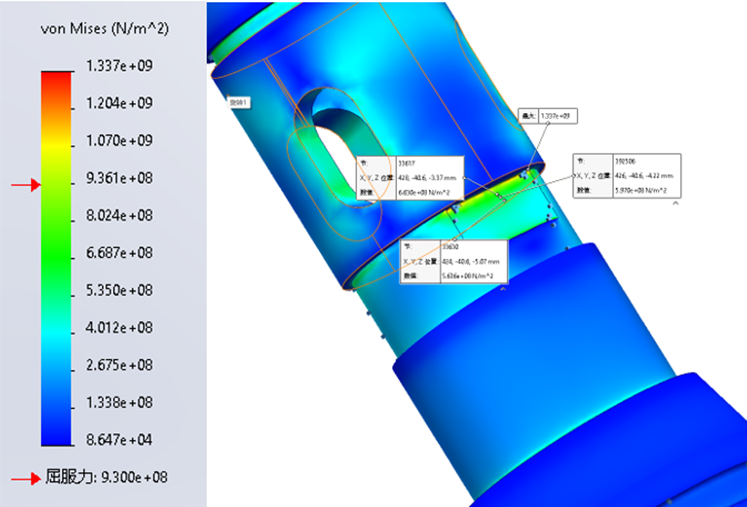
\includegraphics[width=0.45\linewidth]{figure/simulation/lvchulashen.png}%
        \label{fig:fea_filter_outlet_tension}
    }
    \hfill
    % 子图 (b)
    \subfloat[滤出接头受扭应力分布]{%
        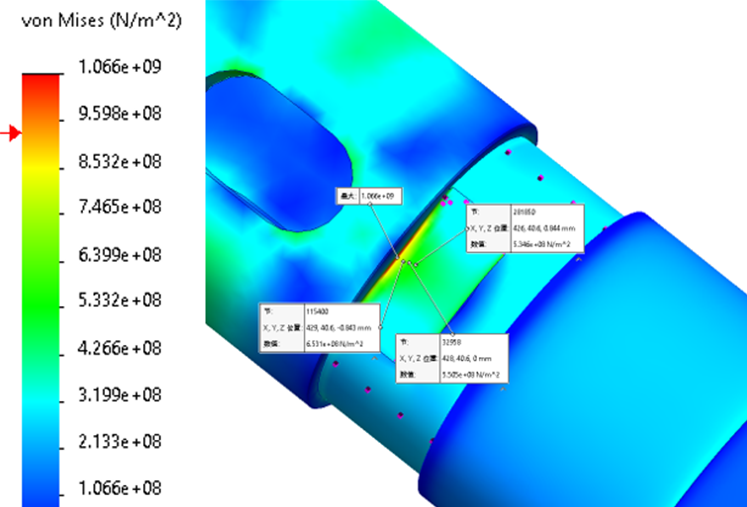
\includegraphics[width=0.45\linewidth]{figure/simulation/lvchuniuju.png}%
        \label{fig:fea_filter_outlet_torsion}
    }
    \vspace{1em}
      % 子图 (c)
    \subfloat[滤进接头受拉应力分布]{%
        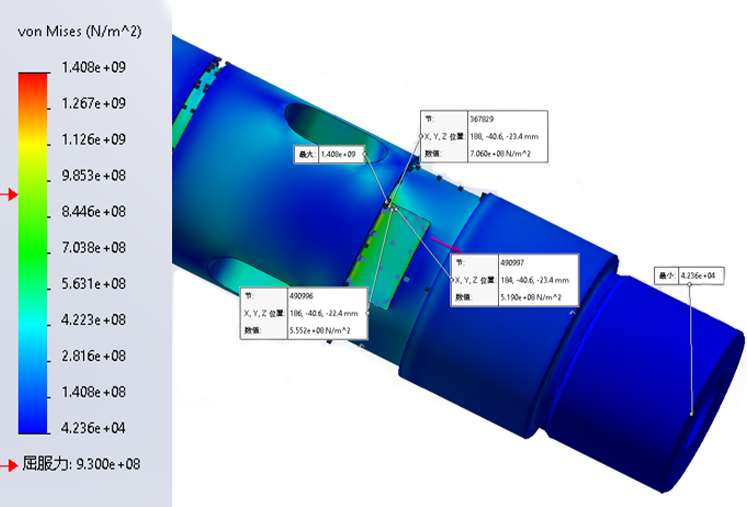
\includegraphics[width=0.45\linewidth]{figure/simulation/lvjinlashen.png}%
        \label{fig:fea_filter_inlet_tension}
    }
    \hfill
      % 子图 (d)
    \subfloat[滤进接头受扭应力分布]{%
        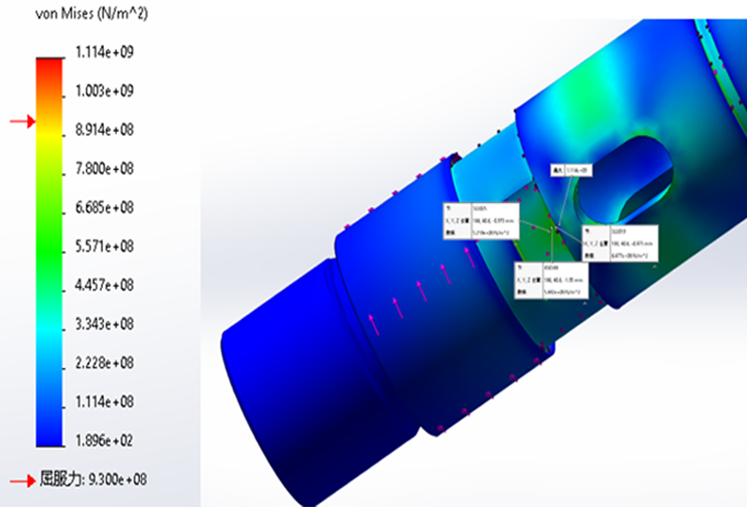
\includegraphics[width=0.45\linewidth]{figure/simulation/lvjinniuju.png}%
        \label{fig:fea_filter_inlet_torsion}
    }
        \caption{过滤工具薄弱零件受载有限元分析结果}
    \label{fig:weak_part_filter_fea}
\end{figure}


\subsubsection{过滤容积计算}

过滤工具容量 $V$ 的计算式为：
\begin{equation}
V = L \cdot A = L \cdot \frac{\pi \cdot (D^2 - d^2)}{4} \times 10^{-6}
\end{equation}
式中，$V$---过滤容量，L（设计指标 $\ge 15$\,L，见本节计算结果）；

$L$---过滤腔长度，mm（取 4864.56\,mm，图号 GLGJ70012A--加长过滤套筒、GLGJ70021A--加长过滤外筒零件图标注的过滤段长度）；

$A$---过滤腔环形截面积，mm$^2$（由过滤外筒内壁与过滤内筒外壁围成的环形面积确定，$A=\pi(D^2-d^2)/4$）；

$D$---过滤腔大径，mm（取 100.26\,mm，图号 GLGJ70021A--加长过滤外筒主视图内孔标注）；

$d$---过滤腔小径，mm（取 73.03\,mm，图号 GLGJ70018A--加长过滤内筒主视图外圆标注）；

$10^{-6}$---量纲换算系数，mm$^3$换算为L（$1\,\text{L} = 10^6\,\text{mm}^3$）。

代入数值计算得：
\begin{equation}
    \begin{aligned}
        V &= L \cdot A = L \cdot \frac{\pi \cdot (D^2 - d^2)}{4} \times 10^{-6} \\
        &= 4864.56 \times \frac{\pi \cdot (100.26^2 - 73.03^2)}{4} \times 10^{-6} \\
        &= 18.0\,\text{L} \ge 15\,\text{L}
    \end{aligned}
\end{equation}
满足设计要求。


各主要受力件的强度校核结果汇总见表~\ref{tab:force_data_filter}。

\begin{table}[htbp]
    \centering
    \caption{受力件数据统计表}
    \label{tab:force_data_filter}
    \renewcommand{\arraystretch}{1.5} % 增加行高，使表格更美观
    \begin{tabularx}{.9\textwidth}{Xc}
        \toprule % 顶线
        受力类型 & 数据 \\
        \midrule % 栏目线
        材料屈服强度 $\sigma_{\mathrm{s}}$ & $930\,\text{MPa}$ \\
        螺纹最大剪切力 $F_{\max1}$ & $1690.3\,\text{kN}$ \\
        NC38接头螺纹最大剪切力 $F_{\max0}$ & $2764.1\,\text{kN}$ \\
        提升短节最大拉力 $F_{\max2}$ & $2838.8\,\text{kN}$ \\
        滤进接头最大拉力 $F_{\max3}$ & $2759.4\,\text{kN}$ \\
        滤出接头最大拉力 $F_{\max4}$ & $2859.0\,\text{kN}$ \\
        下接头最大拉力 $F_{\max5}$ & $2838.8\,\text{kN}$ \\
        材料许用切应力 $[\tau]$ & $613.8\,\text{MPa}$ \\
        最大扭矩（技术参数表许用值） & $39\,\text{kN}\cdot\text{m}$ \\
        提升短节最大扭力 $T_{\max1}$ & $65.6\,\text{kN}\cdot\text{m}$ \\
        滤进接头最大扭力 $T_{\max2}$ & $76.4\,\text{kN}\cdot\text{m}$ \\
        滤出接头最大扭力 $T_{\max3}$ & $78.5\,\text{kN}\cdot\text{m}$ \\
        下接头最大扭力 $T_{\max4}$ & $135.6\,\text{kN}\cdot\text{m}$ \\
        过滤容量 & $18\,\text{L}$ \\
        \bottomrule % 底线
    \end{tabularx}
\end{table}

由表\ref{tab:force_data_filter}可知，过滤工具各受力件的抗拉能力均大于$1000\,\text{kN}$的设计指标（最小为滤出接头凹槽根部$1974.94\,\text{kN}$）；抗扭能力均大于$18\,\text{kN}\cdot\text{m}$的合同指标，其中以提升短节内螺纹根部的$65.6\,\text{kN}\cdot\text{m}$为最小，仍大于技术参数表所列的许用抗扭强度$39\,\text{kN}\cdot\text{m}$，故过滤工具的抗拉、抗扭强度均满足设计要求。


\subsection{操作方式}
\begin{itemize}
	\item 使用时须确保清理盖板处于拧紧状态，避免工具使用中途因清理盖板脱落而导致过滤功能失效。
	\item 清理碎屑时，只需拆卸清理盖板即可，无需拆卸工具本体。
	\item 使用加长版时，需替换过滤套筒、过滤外筒及过滤内筒三个零件，其余零件按原装配方式装配即可。
\end{itemize}


\subsection{维护与保养}

多功能过滤工具每次使用后，应及时清理收集的碎屑，以免影响下一次工具作业；随后用清水清洗各零件，其中上下扶正套筒及清理盖板处需重点清理。工具在井上多次使用或在恶劣条件下工作后，应进行维护修理：全部拆开并更换所有密封件及易损件，检查螺纹及零件是否有损伤，维修完成后重新装配。
